% Für Seitenformatierung

\documentclass[DIV=15]{scrartcl}

% Zeilenumbrüche

\parindent 0pt
\parskip 6pt

% Für deutsche Buchstaben und Synthax

\usepackage[ngerman]{babel}

% Für Auflistung mit speziellen Aufzählungszeichen

\usepackage{paralist}

% zB für \del, \dif und andere Mathebefehle

\usepackage{amsmath}
\usepackage{commath}
\usepackage{amssymb}

% für nicht kursive griechische Buchstaben

\usepackage{txfonts}

% Für \SIunit[]{} und \num in deutschem Stil

\usepackage[output-decimal-marker={,}]{siunitx}
\usepackage[utf8]{inputenc}

% Für \sfrac{}{}, also inline-frac

\usepackage{xfrac}

% Für Einbinden von pdf-Grafiken

\usepackage{graphicx}

% Umfließen von Bildern

\usepackage{floatflt}

% Für Links nach außen und innerhalb des Dokumentes

\usepackage{hyperref}

% Für weitere Farben

\usepackage{color}

% Für Streichen von z.B. $\rightarrow$

\usepackage{centernot}

% Für Befehl \cancel{}

\usepackage{cancel}

% Für Layout von Links

\hypersetup{
	citecolor=black,
	colorlinks=true,
	linkcolor=black,
	urlcolor=blue,
}

% Verschiedene Mathematik-Hilfen

\newcommand \e[1]{\cdot10^{#1}}
\newcommand\p{\partial}

\newcommand\half{\frac 12}
\newcommand\shalf{\sfrac12}

\newcommand\skp[2]{\left\langle#1,#2\right\rangle}
\newcommand\mw[1]{\left\langle#1\right\rangle}
\renewcommand \exp[1]{\mathrm e^{#1}}

% Nabla und Kombinationen von Nabla

\renewcommand\div[1]{\skp{\nabla}{#1}}
\newcommand\rot{\nabla\times}
\newcommand\grad[1]{\nabla#1}
\newcommand\laplace{\triangle}
\newcommand\dalambert{\mathop{{}\Box}\nolimits}

%Für komplexe Zahlen

\renewcommand \i{\mathrm i}
\renewcommand{\Im}{\mathop{{}\mathrm{Im}}\nolimits}
\renewcommand{\Re}{\mathop{{}\mathrm{Re}}\nolimits}

%Für Bra-Ket-Notation

\newcommand\bra[1]{\left\langle#1\right|}
\newcommand\ket[1]{\left|#1\right\rangle}
\newcommand\braket[2]{\left\langle#1\left.\vphantom{#1 #2}\right|#2\right\rangle}
\newcommand\braopket[3]{\left\langle#1\left.\vphantom{#1 #2 #3}\right|#2\left.\vphantom{#1 #2 #3}\right|#3\right\rangle}

\newcommand{\eqnsep}{,\quad}


%\subject{}
\title{physik521 Übung 8}
%\subtitle{}
\author{
    Lino Lemmer
    \and
    Paul Manz
    \and
    Martin Ueding \\ {\small \href{mailto:mu@martin-ueding.de}{mu@martin-ueding.de}}
}

\begin{document}

\maketitle

\newcommand\ZC{Z_\text C}

\section{System von unabhängigen harmonischen Ozsillatoren}

\subsection{Kanonische Zustandssumme}

Zuerst berechnen wir $Z_C$:
\begin{align*}
    Z_\text C
    &= \prod_{n=1}^N \sum_{n_i=0}^\infty \exp\del{- \frac{\hbar\omega \del{n_i + \frac 12}}{kT}} \\
    &= \prod_{n=1}^N \sum_{n_i=0}^\infty \exp\del{- \frac{\hbar\omega}{2kT}} \exp\del{- \frac{\hbar\omega n_i}{kT}} \\
    &= \prod_{n=1}^N \exp\del{- \frac{\hbar\omega}{2kT}} \sum_{n_i=1}^\infty \sbr{\exp\del{- \frac{\hbar\omega}{kT}}}^{n_i} \\
    &= \prod_{n=1}^N \exp\del{- \frac{\hbar\omega}{2kT}} \frac1{1 - \exp\del{- \frac{\hbar\omega}{kT}}} \\
    &= \del{\frac 12 \csch\del{\frac{\hbar\omega}{2kT}}}^N
\end{align*}

Die Energieeigenwerte eines Mikrozustandes $\ket n$ sind einfach die Summen der einzelnen Energieeigenwerte. Und die sind $\hbar\omega\cdot(n + 1/2)$. Oder ist mit $\ket n$ gemeint, dass alle $N$ Oszillatoren den Zustand $n$ haben? Dann ist die Energie einfach $N E_n$.

\subsection{Innere Energie}

Die innere Energie ist der Erwartungswert der Energie:
\begin{align*}
    U
    &= \braket E \\
    &= \sum_{n=0}^\infty W(n) E_n \\
    &= \frac1\ZC \sum_{n=0}^\infty \exp\del{-\frac{E_n}{kT}} E_n \\
    \intertext{%
        Dies schreiben wir jetzt als Ableitung von $\ZC$:
    }
    &= -\frac1\ZC \dpd{}{\frac1{kT}} \sum_{n=0}^\infty \exp\del{-\frac{E_n}{kT}} \\
    \intertext{%
        Das hinter der Ableitung ist gerade $\ZC$. Den Faktor $\frac1\ZC$ ganz
        vorne werden wir noch durch den natürlichen Logarithmus los.
    }
    &= -\dpd{}{\frac1{kT}} \ln(\ZC) \\
    \intertext{%
        Wir transformieren die partielle Ableitung noch mit
        \[
            \dpd{}T = \dpd{\frac1{kT}}T \dpd{}{\frac1{kT}} = - \frac1{kT^2} \dpd{}{\frac1{kT}}
            \implies
            \dpd{}{\frac1{kT}} = - kT^2 \dpd{}T
        \]
        und erhalten so:
    }
    &= kT^2 \dpd{}T \ln(\ZC) \\
    \intertext{%
        Nun setzen wir $\ZC$ ein und führen die Ableitung aus.
    }
    &= NkT^2 \frac{\frac 12 \frac{\hbar\omega}{2 k T^2} \csch\del{\frac{\hbar\omega}{2kT}}\coth\del{\frac{\hbar\omega}{2kT}}}{\frac 12 \csch\del{\frac{\hbar\omega}{2kT}}} \\
    &= N\frac{\hbar\omega}2 \coth\del{\frac{\hbar\omega}{2kT}}
\end{align*}

Wir berechnen den Erwartungswert für die Phononenzahl $n$:
\begin{align*}
    \bracket n
    &= \sum_n W(n) n \\
    &= \frac1\ZC \sum_n \exp\del{-\frac{\hbar \omega \del{n + \frac12}}{kT}} n \\
    \intertext{%
        Wir ziehen $\ZC$ unter alles.
    }
    &= \frac{\sum_n \exp\del{-\frac{\hbar \omega \del{n + \frac12}}{kT}} n}{\ZC} \\
    \intertext{%
        Wir schreiben $\ZC$ aus.
    }
    &= \frac{\sum_n \exp\del{-\frac{\hbar \omega \del{n + \frac12}}{kT}} n}{\sum_n \exp\del{-\frac{\hbar \omega \del{n + \frac12}}{kT}}} \\
    \intertext{%
        Nun addieren wir null.
    }
    &= \frac{\sum_n \exp\del{-\frac{\hbar \omega \del{n + \frac12}}{kT}} n}{\sum_n \exp\del{-\frac{\hbar \omega \del{n + \frac12}}{kT}}} + \frac12 - \frac12 \\
    \intertext{%
        Die $+\frac 12$ werden in den Zähler integriert.
    }
    &= \frac{\sum_n \exp\del{-\frac{\hbar \omega \del{n + \frac12}}{kT}} \del{n + \frac12}}{\sum_n \exp\del{-\frac{\hbar \omega \del{n + \frac12}}{kT}}} - \frac12 \\
    \intertext{%
        Wir wenden den Trick mit der Ableitung an und ziehen somit das $(n +
        \frac 12)$ in die Ableitung rein.
    }
    &= - \frac{\dpd{}{\frac{\hbar\omega}{kT}} \sum_n \exp\del{-\frac{\hbar \omega \del{n + \frac12} }{kT}}}{\sum_n \exp\del{-\frac{\hbar \omega \del{n + \frac12}}{kT}}} - \frac12 \\
    \intertext{%
        Das ganze können wir auch als Ableitung einer Logarithmusfunktion
        schreiben.
    }
    &= - \dpd{}{\frac{\hbar\omega}{kT}} \ln\del{\sum_n \exp\del{-\frac{\hbar \omega \del{n + \frac12}}{kT}}} - \frac12 \\
    \intertext{%
        Dies ist gerade $Z_{\text C,1}$.
    }
    &= -\dpd{}{\frac{\hbar\omega}{kT}} \ln(Z_{\text C,1}) - \frac12 \\
    \intertext{%
        Wir setzen unser vorheriges Ergebnis für $Z_{\text C,1}$ ein.
    }
    &= \dpd{}{\frac{\hbar\omega}{kT}} \ln\del{2 \sinh\del{\frac{\hbar\omega}{2kT}}} - \frac12 \\
    \intertext{%
        Die Ableitung führen wir aus:
    }
    &= \frac{2 \cosh(\ldots)}{2 \sinh(\ldots)} \frac 12 - \frac 12 \\
    \intertext{%
        Wir benutzen die Exponentialdarstellung der Funktionen.
    }
    &= \frac 12\del{\frac{\eup^{\ldots} + \eup^{-\ldots}}{\eup^{\ldots} - \eup^{-\ldots}} - \frac 12} \\
    \intertext{%
        Nach etwas umstellen erhalten wir:
    }
    &= \frac1{\exp\del{\frac{\hbar\omega}{kT}} - 1}
\end{align*}

Dies ist der gesuchte Erwartungswert.

Wir können nun das Zwischenergebnis benutzen, um die innere Energie noch etwas kompakter auszudrücken. Dieses Ergebnis ist:
\[
    \braket n = \frac12 \coth\del{\frac{\hbar\omega}{2kT}} - \frac 12
\]

Unsere bisherige Form für die innere Energie ist:
\begin{equation}
    \label{eq:U}
    U = N \frac{\hbar\omega}2 \coth\del{\frac{\hbar\omega}{2kT}}
\end{equation}

Dies können wir jetzt benutzen, um zu schreiben:
\[
    U = N \hbar \omega \del{\bracket n + \frac12}
\]

Wir benutzen die Form \eqref{eq:U}, um die Abhängigkeit der inneren Energie von $kT/\hbar\omega$ zu plotten. Dies ist in Abbildung~\ref{fig:U} dargestellt.

\begin{figure}[htbp]
    \centering
    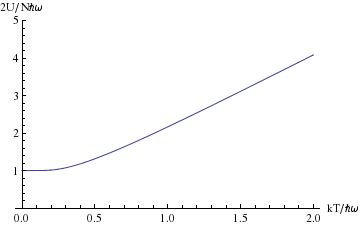
\includegraphics[width=.6\linewidth]{2b.png}
    \caption{%
        Abhängigkeit der inneren Energie von $kT/\hbar\omega$.
    }
    \label{fig:U}
\end{figure}

\subsection{Freie Energie}

Die freie Energie errechnen wir aus der Zustandssumme:
\begin{align*}
    F
    &= - k T \ln(\ZC) \\
    &= - N k T \ln\del{\frac 12 \csch\del{\frac{\hbar\omega}{2kT}}} \\
    &= N k T \ln\del{2 \sinh\del{\frac{\hbar\omega}{2kT}}} \\
    \intertext{%
        Im Skript ist jetzt noch mit Formel (4.77) eine weitere Umformung
        gemacht:
    }
    &= N \del{kT \ln\del{1 - \exp\del{-\frac{\hbar\omega}{kT}}} + \frac{\hbar\omega}2}
\end{align*}

Aus der zweiten Zeile berechnen die Entropie durch Ableitung nach der Temperatur:
\begin{align*}
    S
    &= - \dpd FT \\
    &= - N \frac{\hbar\omega}{2T} \coth\del{-\frac{\hbar\omega}{kT}} + N k \ln\del{\frac 12 \csch\del{-\frac{\hbar\omega}{kT}}}
\end{align*}

Somit erhalten wir:
\[
    TS = - N \frac{\hbar\omega}{2} \coth\del{-\frac{\hbar\omega}{kT}} + N k T \ln\del{\frac 12 \csch\del{-\frac{\hbar\omega}{kT}}}
\]

Mit $U = F + TS$ erhalten wir dann als innere Energie
\[
    U = N \frac{\hbar\omega}{2} \coth\del{\frac{\hbar\omega}{kT}},
\]
in Übereinstimmung mit \eqref{eq:U}.

\subsection{Ausdruck für die Wärmekapazität}

In Abbildung~\ref{fig:1d-c} ist dieses Verhalten dargestellt.

\begin{figure}[htbp]
    \centering
    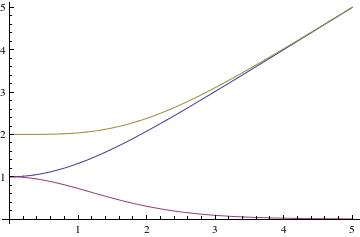
\includegraphics[width=0.6\linewidth]{1d.png}
    \caption{%
        Wärmekapazität $c$ in Einheiten von $k$ gegen $\hbar\omega / kT$. Die
        violette Linie ist der erste Summand, die Blaue der Zweite und die
        Gelbe die Summe der beiden.
    }
    \label{fig:1d-c}
\end{figure}

\section{Gibb'sches Paradoxon}

\subsection{Druck- und Temperaturausgleich}

Gegeben sind:
\[
    N_1
    \eqnsep
    N_2
    \eqnsep
    p_1
    \eqnsep
    p_2
    \eqnsep
    T_1
    \eqnsep
    T_2
\]
Da wir ideale Gase betrachten gilt zunächst:
\begin{align*}
p_1V_1 &= N_1k_\text B T_1 \\
p_2V_2 &= N_2k_\text B T_2 \\
U &= \frac{3}{2}N_1 k_\text B T_1 + \frac{3}{2} N_2 k_\text BT_2
\end{align*}

Die innere Energie bleibt beim Gesamtprozess erhalten:
\begin{align*}
U = \frac{3}{2} N_1 k_\text B T_1 + \frac{3}{2}N_2 k_\text B T_2 &= \frac{3}{2}(N_1+N_2) k_\text B T \\
\implies \del{N_1+N_2} k_\text BT &= N_1 k_\text B T_1 + N_2 k_\text B T_2 \\
\end{align*}
Gemäß idealer Gasgleichung gilt im Endzustand aber:
\[p\del{V_1+V_2}=\del{N_1+N_2}k_\text BT \]
Setzt man ein, erhält man:
\begin{align*}
p\del{V_1+V_2} &= N_1k_\text BT_1+N_2k_\text BT_2 \\
\implies p &= \frac{N_1k_\text BT_1 + N_2k_\text BT_2}{V_1+V_2} \\
\implies T &= \frac{p}{\del{N_1+N_2}k_\text B}=\frac{N_1T_1 + N_2T_2}{\del{V_1+V_2}\del{N_1+N_2}}
\end{align*}


\subsection{Änderung der Entropie}
Die Entropie vor Entfernen der Trennwand ist:
\[ S = N_1 k_\text B \del{\ln V_1 +\frac{3}{2}\del{1+\ln\del{2\pi m_1 k_\text B T /h^2}}}  + N_2 k_\text B \del{\ln V_2 +\frac{3}{2}\del{1+\ln\del{2\pi m_2 k_\text B T /h^2}}} \]
Nach Entfernen der Trennwand sind die Gasteilchen beider Sorten auf das Gesamtvolumen verteilt, für die Entropie ergibt sich:
\[ S' = N_1 k_\text B \del{\ln V +\frac{3}{2}\del{1+\ln\del{2\pi m_1 k_\text B T /h^2}}}  + N_2 k_\text B \del{\ln V +\frac{3}{2}\del{1+\ln\del{2\pi m_2 k_\text B T /h^2}}} \]
Die Differenz der beiden Ausdrücke ergibt:
\[\Delta S = N_1 k_\text B \ln V - N_1 k_\text B \ln V_1 + N_2 k_\text B \ln V - N_2 k_\text B \ln V_2 = N_1 k_\text B \ln\del{\frac{V_1+V_2}{V_1}} + N_2 k_\text B \ln\del{\frac{V_1+V_2}{V_2}} > 0 \]
Auch im Falle identischer Teilchen würde sich dabei die Entropie erhöhen, obwohl es zu keiner Zustandsänderung gekommen ist. Das steht im Widerspruch zur Tatsache, dass die Entropie eine Zustandsvariable ist und damit für einen bestimmten Zustand eindeutig ist.

\section{Maxwell'sche Geschwindigkeitsverteilung}

\subsection{Wahrscheinlichkeitsdichte}
Gesucht ist die Wahrscheinlichkeitsdichte des Geschwindigkeitsbetrags eines Teilchens. Die kinetische Energie ist gegeben durch
\[T=\frac{mv^2}{2}.\]
Damit ergibt sich im kanonischen Formalismus eine Wahrscheinlichkeitsdichte von
\[W(v) \dif v = \frac{4\pi v^2}{Z_\text c} \exp\del{-\frac{\beta mv^2}{2}} \dif v, \]
wobei sich der Faktor $4\pi v^2$ durch die Jacobideterminante bei der Betrachtung
Für die Normierung muss die Dichte über alle Geschwindigkeiten integriert werden:
\begin{align*}
Z_\text c &= \int \dif{}^3v \exp\del{-\frac{\beta m\vec{v}^2}{2}} \\
&= \int\dif v_1 \int\dif v_2 \int\dif v_3 \exp\del{-\frac{\beta m \del{ v_1^2+v_2^2+v_3^2}}{2}} \\
&= \del{\int \dif v \exp\del{-\frac{\beta m{v}^2}{2}}}^3 \\
&= \del{\sqrt{\frac{2\pi}{\beta m}}}^3
\end{align*}
Daraus folgt also:
\[W(v) \dif v = \sqrt{\frac{2}{\pi}} \del{\frac{m}{k_\text B T}}^{3/2} v^2 \exp\del{-\frac{mv^2}{2k_\text BT}} \dif v \]

\subsection{Mittlere und wahrscheinlichste Geschwindigkeit}
Berechne die mittlere Geschwindigkeit:
\begin{align*}
\bar{v} &= \int \dif v \ \rho(v) v \\
&= \int_0^\infty \dif v \ \frac{4\pi v^3}{Z_\text C} \exp\del{-\frac{mv^2}{2k_\text B T}} \\
&= \int_0^\infty \dif q \ \frac{q}{2Z_\text C} \exp\del{-\frac{mq}{2k_\text B T}} \\
&= \int_0^\infty \dif q \ \frac{1}{2Z_\text C} \exp\del{-\frac{mq}{2k_\text B T}}\del{-\frac{-2k_\text B T}{m}} \\
&= \frac{1}{2Z_\text C}\del{\frac{-2k_\text B T}{m}}^2 \\
&= \sqrt{\frac{8k_\text B T}{\pi m}}
\end{align*}

Berechne die wahrscheinlichste Geschwindigkeit. Diese ist durch das Maximum der Wahscheinlichkeitsdichte gegeben, es muss also gelten:
\[\frac{\dif}{\dif v}W(v)\bigg|_{v=v_W}=0\]
\begin{align*}
\frac{\dif}{\dif v}W(v) &= \frac{1}{Z_\text C}\del{2v\exp\del{-\frac{mv^2}{2k_\text BT}}-\frac{2v^3m}{2k_\text BT}\exp\del{-\frac{mv^2}{2k_\text BT}}} \\
&= \frac{v}{Z_\text C}\exp\del{-\frac{mv^2}{2k_\text BT}} \del{2-\frac{v^2m}{k_\text B T}} \stackrel{!}{=} 0 \\
\end{align*}
$W(v)$ ist nur für positive $v$ definiert und $W(0)=0$. Für die wahrscheinlichste Geschwindigkeit bleibt also nur noch übrig:
\[v_\text W=\sqrt{\frac{2k_\text BT}{m}}\]

\subsection{Weitere Freiheitsgrade}
Da Rotations- und Vibrationsfreiheitsgrade nicht mit der Schwerpunktsbewegung der Teilchen wechselwirken können wir die Geschwindigkeitsverteilung für festgehaltene Rotations- bzw Vibrationsenergie betrachten. Sie unterscheidet sich bei zweiatomigen Molekülen also nicht von der Geschwindigkeitsverteilung für Einzelatome.

\IfFileExists{\bibliographyfile}{
    \printbibliography
}{}

\end{document}

% vim: spell spelllang=de
